\color{red}
\subsection{Enabling Side-Channel Aware Software Development}
Most software developers lack both the know-how and the equipment to evaluate
their software's potential vulnerability to analog side channels.  As such,
blackbox software which enables developers to analyze their software for analog
side channels is valuable. To enable this type of software analysis, we have
developed a framework which performs symbolic execution of a program on a
detailed (gate-level) model of a microprocessor~\cite{cherupalli2017}.
This framework was originally developed in order to automate design of
`bespoke microprocessors' --- microprocessors designed to execute a single
application binary. The flowchart for this use case is in Fig.~\ref{fig:bespoke}.
The symbolic execution of the program on the hardware occurs in the
`Gate Activity Analysis' stage.

\begin{wrapfigure}{l}{0.4\linewidth}
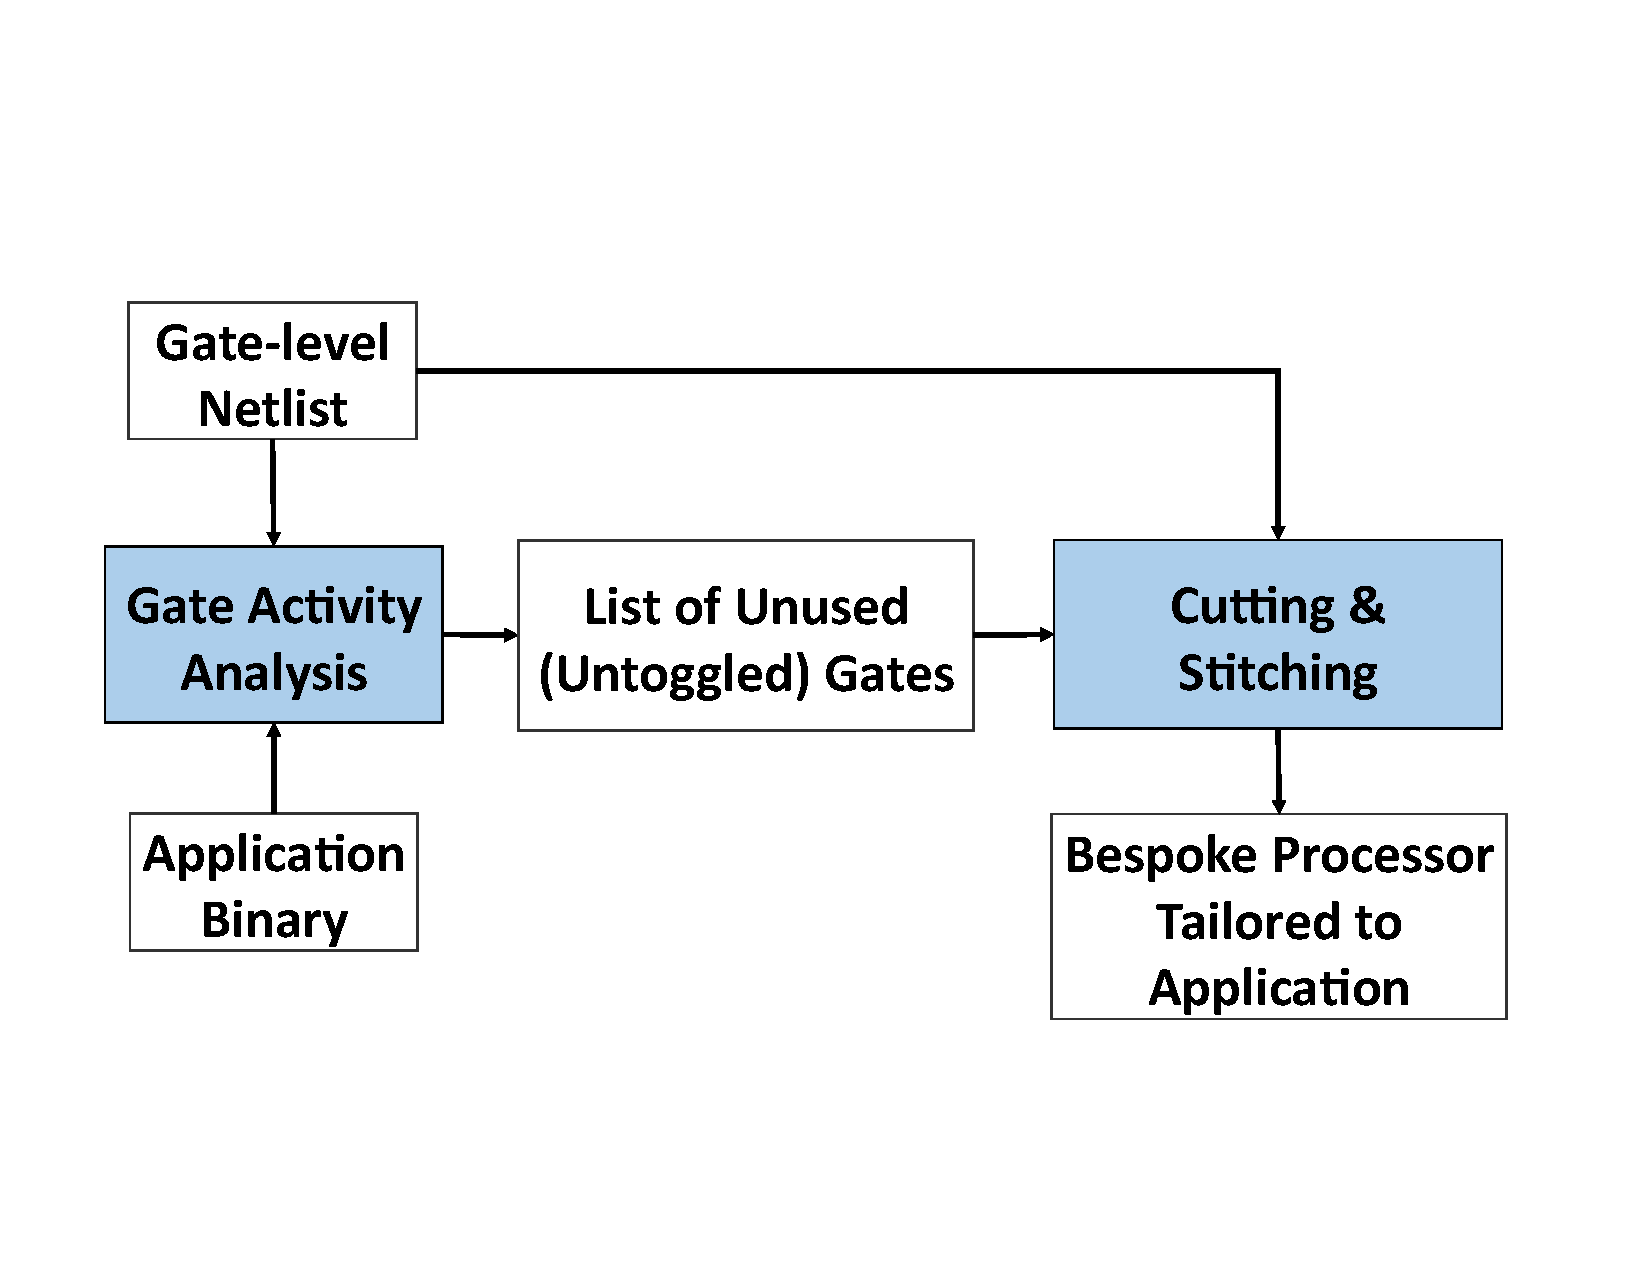
\includegraphics[width=\linewidth]{./figure/Bespoke_Flow_Fig.pdf}
\caption{\small
    Hardware-software co-analysis used to generate bespoke microprocessors.}
\label{fig:bespoke}
\end{wrapfigure}

Program execution is affected by program inputs (e.g., sensor inputs) and
different inputs can result in not just variation in data-dependent activities
(i.e., switching activities on data and address busses), but also variation in
instruction-dependent activities due to input-dependent branch instructions.
This symbolic execution framework allows us to identify whether any possible
execution of a program leads to an EM side-channel which leaks sensitive
information. Security is a critical consideration for processors in the IoT
space.
However, many IoT devices cannot afford to run advanced security
protocols due to energy constraints. Our symbolic execution framework will
allow us to identify when a program is susceptible, and, importantly, when it
is not susceptible to an EM side-channel attack, allowing us to add or remove
the often expensive software based techniques to mitigate side-channel attacks
as needed.

Our framework has shown applicability for security
applications~\cite{cherupalli20172}. We have demonstrated its use in
taint-tracking for information flow security to locate information policy
violations, even violations which result from covert timing side-channels.

\color{black}
